\section{L'implementazione del database}
Nelle sezioni precedenti si è discusso delle proprietà
offerte dai diversi tipi di database e
delle necessità che il dominio impone sul sistema.
La scelta del database deriva quindi dall'incrocio di tutte queste condizioni,
individuando la tecnologia che meglio riesce a rispondere alle esigenze del progetto.
Ogni tipologia di database comporta un approccio differente alle informazioni,
implicando una strategia di salvataggio e manipolazione dei dati propria.
Le strutture che modellano le entità devono quindi
essere create per sfruttare nella maniera più efficiente possibile
i vantaggi offerti dalla tecnologia scelta.\\
\\
Una volta scelto il database e le strutture in base alla modalità
che più si addicono alle esigenze del progetto,
l'utilizzo di servizi in cloud comporta una maggiore attenzione anche
alle proprietà legate al mantenimento del servizio,
dalle quali derivano le proprietà di scalabilità e affidabilità.
La grande differenza tra i vari servizi sta nelle proprietà del server
incaricato di fornire il potere computazionale necessario per l’esecuzione.
L’architettura del server e la sua integrazione con la tecnologia del database
determinano infatti l’effettiva capacità di scalabilità del servizio.\\
\\
Si intende scalabilità verticale la capacità di aumentare le risorse
della stessa macchina in cui si esegue il codice.
La scalabilità verticale viene definita nel momento di creazione del servizio,
in cui si determinano le risorse da dedicare alla macchina che esegue il programma.
Trattandosi di macchine virtualizzate,
è sempre possibile in un secondo momento aumentare le prestazioni in caso di necessità.\\
\\
Per scalabilità orizzontale si intende invece la capacità di
delegare il carico di lavoro ad altre macchine, eventualmente coordinando le modifiche.
Questo permette una risposta alle richieste più resistente,
riducendo il rischio di colli di bottiglia che potrebbero venirsi a formare nell’utilizzo di un nodo singolo.
La scalabilità orizzontale richiede però l'implementazione
di tecnologie apposite integrate con il database che permettano l'esecuzione in nodi fisici differenti. \\
\\
Una volta individuata la tecnologia adatta e il livello di scalabilità desiderati,
è bene considerare le altre necessità o le opportunità aggiuntive generate
dalla presenza di un database nel progetto. \\
\\
L’alta disponibilità(HA) è la proprietà di garantire l’accesso al servizio nonostante i guasti.
Ad esempio, si può mantenere una macchina identica al server principale in grado di replicare il servizio,
spostando il carico in caso di guasto del server principale.
Si misura in “numero di nove”, ovvero la quantità di nove presenti
nella percentuale del tempo per il quale si garantisce la disponibilità del servizio.
I servizi offrono diverse qualità di HA, in base alle funzionalità desiderate.\\
\\
Alcuni servizi possono presentare offerte di backup
per riportare il server nello stesso stato di qualche momento precedente.
Questo permette il ripristino del sistema a un punto precedente
rispetto all'avvenimento di eventuali errori o guasti del sistema.\\
\subsection{La scelta del database}

Viste le necessità del progetto in ambito di scalabilità
e le caratteristiche del dominio,
si individua nei database documentali la tecnologia più adatta
per gestire la persistenza centrale dell'applicazione.\\
\\
I database documentali, facenti parte della categoria dei database non relazionali,
rappresentano un paradigma di gestione dei dati
che organizza le informazioni in documenti.
Ogni documento è un'unità autonoma che incapsula la descrizione di un'entità,
contenendo le sue proprietà.
Tali documenti sono logicamente raggruppati in collezioni.
All'interno di una collezione,
ciascun documento è univocamente identificato da un proprio identificativo,
garantendo l'accesso diretto e la manipolazione individuale.\\
\\
Un aspetto distintivo e strategicamente rilevante dei database documentali è
la loro intrinseca capacità di supportare la scalabilità orizzontale in modo nativo.
Questo è un vantaggio fondamentale in architetture distribuite e ambienti ad alta intensità di dati.
La scalabilità è realizzata attraverso la partizionamento (o sharding),
un meccanismo che distribuisce automaticamente i dati tra diversi nodi di archiviazione fisici.\\
\\
Attraverso la denormalizzazione si possono migliorare le prestazioni di lettura,
aggregando dati correlati all'interno di un singolo documento o partizione.
Questo approccio semplifica la gestione delle join,
che possono essere ottimizzate per risiedere all'interno della stessa partizione o
in partizioni vicine, minimizzando la necessità di operazioni di lettura tra nodi distinti.\\
\\
La denormalizzazione comporta intrinsecamente
alcune sfide a livello di consistenza dei dati,
in particolare per le operazioni di recupero che coinvolgono dati potenzialmente duplicati.
Questo problema è efficacemente mitigato dall'adozione di Global Secondary Indexes (GSI).
I GSI consentono di interrogare i dati su attributi che non sono la chiave primaria del documento,
e risiedono quindi su partizioni differenti.
Forniscono percorsi di accesso alternativi e performanti sull'intero dataset distribuito,
superando le limitazioni imposte dalla distribuzione fisica delle partizioni e
mantenendo un'elevata efficienza nelle query complesse.\\
\\
Implementando automaticamente e nativamente la scalabilità orizzontale,
il database relazionale ci permette quindi di gestire con efficienza
l'incremento dei volumi di dati e dei carichi di lavoro senza interventi complessi.
Fornisce inoltre un supporto diretto all'esigenza dell'architettura
riguardo alla necessita di letture performanti
da entrambi i lati di relazioni molti-a-molti:
attraverso il partizionamento strategico,
i dati correlati possono essere collocati in partizioni vicine
per ottimizzare le letture da un lato della relazione,
mentre i Global Secondary Indexes (GSI) superano le limitazioni delle partizioni fisiche,
consentendo interrogazioni efficienti e performanti dall'altro lato.
Infine, un'attenta progettazione del modello di dati,
che include una denormalizzazione strategica e l'utilizzo degli indici,
garantirà un tempo di recupero ridotto per le informazioni,
massimizzando la reattività del sistema e l'efficienza complessiva.\\
\\
Un confronto con il paradigma relazionale evidenzia le ragioni della sua esclusione per le esigenze del nostro progetto.
Sebbene i database relazionali siano soluzioni consolidate per la gestione di dati strutturati,
presentano delle limitazioni che non si allineano con i requisiti di scalabilità richiesti.
La loro architettura, che spesso lega indici e tabelle alla stessa partizione logica,
impone intrinsecamente dei vincoli sulla scalabilità orizzontale,
non solo per la difficoltà di distribuire indici e tabelle su nodi diversi,
ma anche per il numero massimo di connessioni contemporanee che possono gestire,
limitando la capacità di rispondere a un numero massiccio di richieste simultanee.
L'implementazione dello sharding, sebbene possibile, è interamente a carico dello sviluppatore,
introducendo un significativo onere di progettazione, sviluppo e manutenzione.\\
\\
Inoltre, la gestione di relazioni molti-a-molti nel modello relazionale,
pur essendo logicamente chiara con tabelle di giunzione,
può presentare problemi di scalabilità in contesti di elevato carico.
Quando una query necessita di recuperare dati da entrambi i lati di una relazione molti-a-molti,
ciò implica l'esecuzione di join complesse tra più tabelle.
Sebbene queste operazioni possano essere veloci su singole istanze di database ben ottimizzate,
in un ambiente distribuito e con volumi di dati in crescita,
queste join possono richiedere il trasferimento di grandi quantità di dati tra nodi diversi per essere risolte,
introducendo latenza e overhead di rete significativi.
Questo può diventare un collo di bottiglia, compromettendo le performance complessive.
Infine, la mancanza di un supporto nativo per indici secondari globali (GSI)
rende più complessa la gestione di query su attributi non chiave distribuiti su diverse partizioni,
costringendo a soluzioni alternative che potrebbero compromettere
la reattività del sistema e aumentare la complessità del codice.
Questi fattori combinati ci hanno portato a escludere il modello relazionale.\\
\\
Essendo il progetto già improntato sulla piattaforma Azure,
la ricerca verte inizialmente tra le opzioni che mette a disposizione.
Azure offre un’ampia scelta di database documentali che possono essere integrati con il resto dell’ecosistema.
Tuttavia, Azure presenta un servizio completamente gestito e nativo
per i database non relazionali chiamato Azure Cosmos DB.
Garantendo la massima interoperabilità all'interno dell'ecosistema,
si procede analizzando le proprietà e i vantaggi offerti da Cosmos DB.\\
\\
Azure Cosmos DB si distingue per la sua capacità di scalare orizzontalmente in maniera illimitata,
consentendo di gestire volumi di dati e carichi di lavoro molto elevati,
fino a milioni di richieste al secondo,
grazie alla possibilità di distribuire il carico à su più regioni Azure.
È stato infatti ideato per essere presentare un'architettura distribuita,
con replica automatica dei dati,
assicurando un'elevatissima disponibilità e resilienza.
Queste vengono assicurate anche in caso di interruzioni regionali,
grazie a meccanismi di failover automatico.
Inoltre, la distribuzione globale "turnkey" garantisce che i dati siano sempre vicini agli utenti,
riducendo drasticamente la latenza a millisecondi a cifra singola
(con SLA del 99.999\% di disponibilità per account multi-regione).
Consente l'indicizzazione attraverso più partizioni in maniera
automatica e personalizzabile ottimizzado le query,
riducendo la complessità e migliorando le prestazioni,
senza richiedere oneri di gestione manuale degli indici.\\
\begin{figure}[h!]
    \centering
    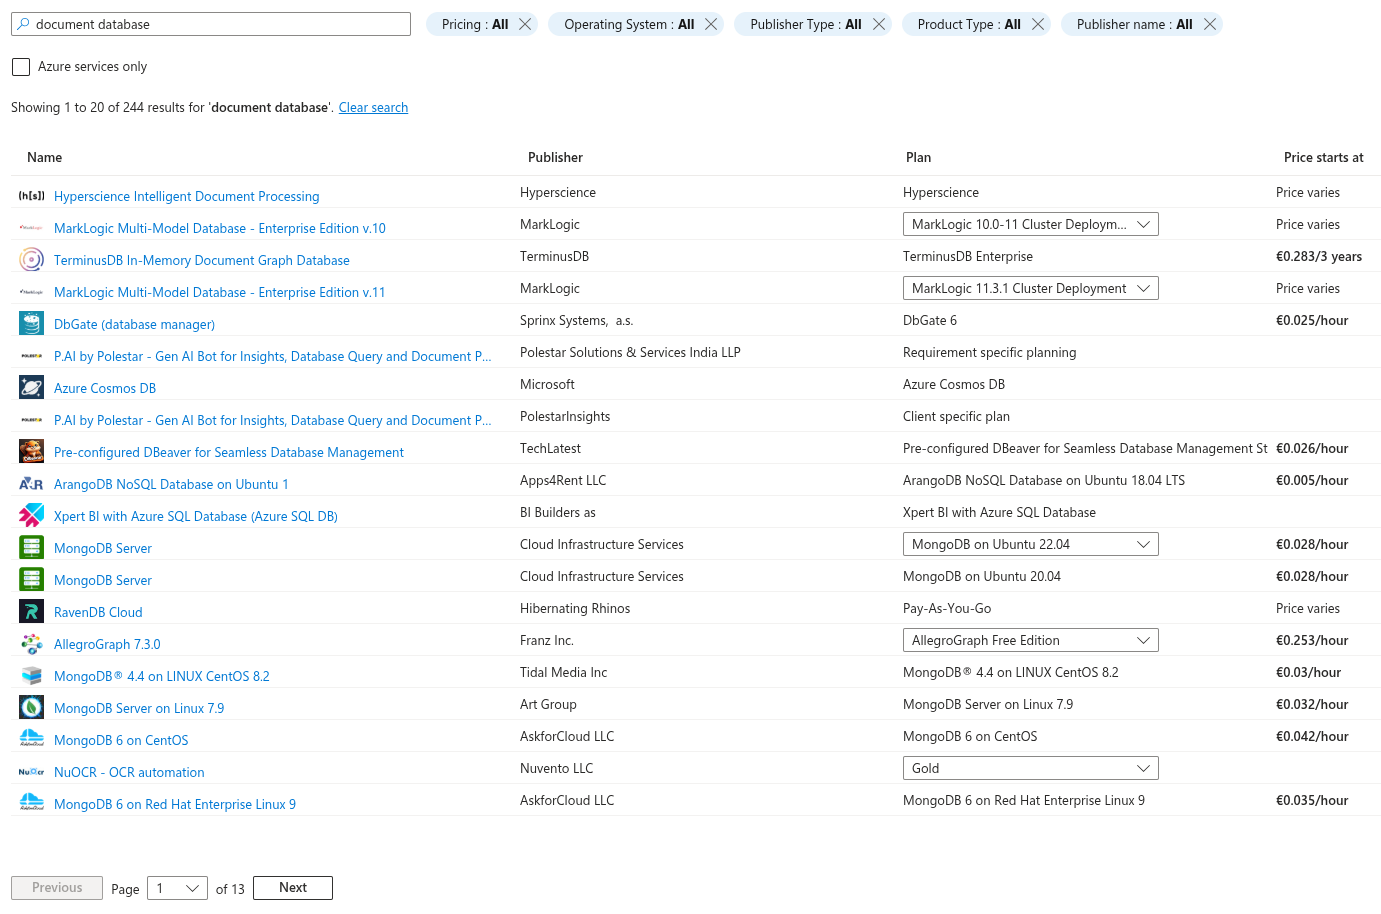
\includegraphics[width=\textwidth]{AzureDatabase.png}
    \caption{Proposte di Azure per i database documentali}
\end{figure}


\begin{wrapfigure}{r}{0.25\textwidth}
    \centering
    
\includegraphics[height=.12\textheight]{cosmos.png}
    Azure Cosmos
\end{wrapfigure}
Pur essendo focalizzato sui database documentali,
Cosmos DB è però una soluzione multi-modello e multi-API.
Supporta infatti, oltre alla sua API nativa per NoSQL (che usa il modello a documenti JSON),
anche API compatibili con MongoDB, Apache Cassandra, Apache Gremlin (per i grafi) e Azure Table.
Questa versatilità permette agli sviluppatori di utilizzare strumenti familiari,
semplificando la migrazione di applicazioni esistenti o
lo sviluppo di nuove con la flessibilità di scegliere il modello di dati più appropriato.\\
\\
A livello di costi è difficile portare un'analisi precisa,
in quanto tutti i competitor presentano servizi
con capacità, disponibilità e intregrazione differenti.
I modelli di pagamento che utilizzano metriche di utilizzo diverse,
rendendo necessarie ulteriori analisi che dipendono anche
dall'effettiva tipologia e quantità delle richieste che vertono sul database.
Di seguito viene riportata una tabella per comparazione i costi delle alternative principali.
Cosmos usa come metrica le Rerquest Units(RU) per quantificare l'impatto di una richiesta sul database.
Le RU rappresentano un'astrazione delle risorse di sistema (CPU, I/O, memoria).
Ogni operazione consuma RU, proporzionalmente alla sua
complessità, dimensione e al carico computazionale richiesto.\\

\begin{longtable}{|P{3.2cm}|P{4.2cm}|P{4.2cm}|P{3cm}|}
    \hline
    \textbf{Servizio}      & \textbf{Costo ogni milione di scritture}\newline(normalizzate a 1 KB) & \textbf{Costo ogni milione di scritture}\newline (normalizzate a 1 KB) & \textbf{Costo di manutenzione GB/mese} \\
    \hline
    AWS DynamoDB           & \$1.25                                                                & \$0.25                                                                 & \$0.25                                 \\
    \hline
    Google Cloud Firestore & \$0.90                                                                & \$0.30                                                                 & \$0.156                                \\
    \hline
    Azure Cosmos DB        & In base al consumo di RU, \$5.84 al mese ogni 100RU/s                 & In base al consumo di RU, \$5.84 al mese ogni 100RU/s                  & \$0.25 (Transazionale)                 \\
    \hline
    \caption{Costi dei principali database documentali gestiti in Cloud}
\end{longtable}

La difficoltà di stabilirne il costo in una fase iniziale
è mitigata però dalla presenza di un piano gratuito perenne.
Cosmos DB offre infatti una quota gratuita di risorse iniziali,
per tutta la durata dell'utilizzo.
Il piano prevede 25 GigaByte di memoria gratuita,
a cui si aggiungono 1000 RU/s offerti per ogni categoria di operazione, 
suddivise in lettura, scrittura e eliminazione. 
Dato lo stadio iniziale del progetto queste caratteristiche sono state considerate sufficenti,
permettendo di sfruttare e testare le capacità di distribuzione.
Nel caso in cui, in una fase sucessiva del progetto,

In caso ulteriori analisi svolte sucessivamente nel progetto,
(grazie ai dati dell'utilizzo effettivo)
non identifichino questa soluzione come la più adatta, 

"Qualora, in seguito a ulteriori analisi condotte nelle fasi successive del progetto — rese possibili dai dati derivanti dall’utilizzo effettivo del sistema — emergesse che la soluzione adottata non rappresenta l’opzione più adeguata, sarà possibile valutarne l’evoluzione o la sostituzione con alternative più rispondenti ai requisiti osservati."

lo spostamento dei dati verso un altro gestore richiede uno sforzo limitato,
data la compatibilità nella raprresentazione dei dati tra le diverse tecnologie di database documentali.\\
\\
impostazioni di cosmos\\
\\


Inoltre, Azure mette a disposizione molteplici servizi accessori che possono essere uniti al servizio.
Questo permette di estendere le potenzialità del database tramite  l’analisi e il monitoraggio dei dati,
generando prestazioni aggiuntive o integrando i dati per lo sviluppo di altre tecnologie.\\
\\

Al server principale è stata affiancata una replica che rimane costantemente aggiornata.
Situata in una località differente dal server principale,
garantisce alta disponibilità continuando a fornire i servizi anche in caso di malfunzionamenti al server principale.\\
\\

Nel caso in cui però fossero necessarie ulteriori prestazioni,
se il dominio e i requisiti lo permettono,
si può eventualmente delegare a un database non relazionale le modifiche ai dati e alle relazioni
che non necessitano delle qualità ACID ma richiedono un’alta frequenza di scrittura.\\
\\
Interporre una cache tra la logica applicativa e il database
semplifica e riduce il numero di richieste verso il database.
Il livello di caching si occupa di gestire le richieste al database
fornendo e duplicando le risposte che possiede già in memoria,
eventualmente concentrando le richieste in caso i dati siano invece da recuperare.
Per i dati in scrittura, invece, salva temporaneamente le modifiche richieste,
aggiornando subito la memoria locale,
per poi apportare le modifiche al database in momenti di carico ridotto.
Garantisce così un tempo di risposta e di propagazione degli aggiornamenti ridotto,
alleviando il numero di richieste al database, estendendo così  le prestazioni fornite.\\
\\


Tuttavia, non vi è alcun vincolo che impedisca l'affiancamento di database di tipologia diversa
per rispondere a esigenze specifiche e sfruttare i punti di forza di entrambe le tecnologie.
\\

\subsection{La definizione delle classi}
Nonostante sia più probabile che venga richiesto il dettaglio di un evento,
e quindi sia più frequente il dover recuperare i Profile relativi all’Event,
la proporzione delle richieste prevista non giustifica lo sbilanciamento della relazione sugli Event.
Infatti, se si salvassero tutti i ProfileEvent sull’oggetto Event,
le richieste degli eventi appartenenti ai profili, sebbene meno frequenti,
richiederebbero l’ispezione di tutti gli Event alla ricerca del Profile indicato.
Infine, se si duplicasse l’oggetto ProfileEvent,
oltre che nella sua tabella originaria, anche sugli Event la sua creazione,
la sua eliminazione e la modifica del campo Confirmed richiederebbero il doppio delle scritture.\\
\\



\subsection{L'integrazione con le Azure Functions: il framework .Net e l'eventual consistency}

\clearpage




\clearpage




\subsection{L' integrazione con C\#}

La scelta di un database relazionale per la persistenza ha comportato sviluppi progettuali precisi.
In primis si rende necessario tradurre il dominio in componenti relazionali che possano essere espressi e salvati nelle tabelle del database.

\begin{figure}[h!]
    \centering
    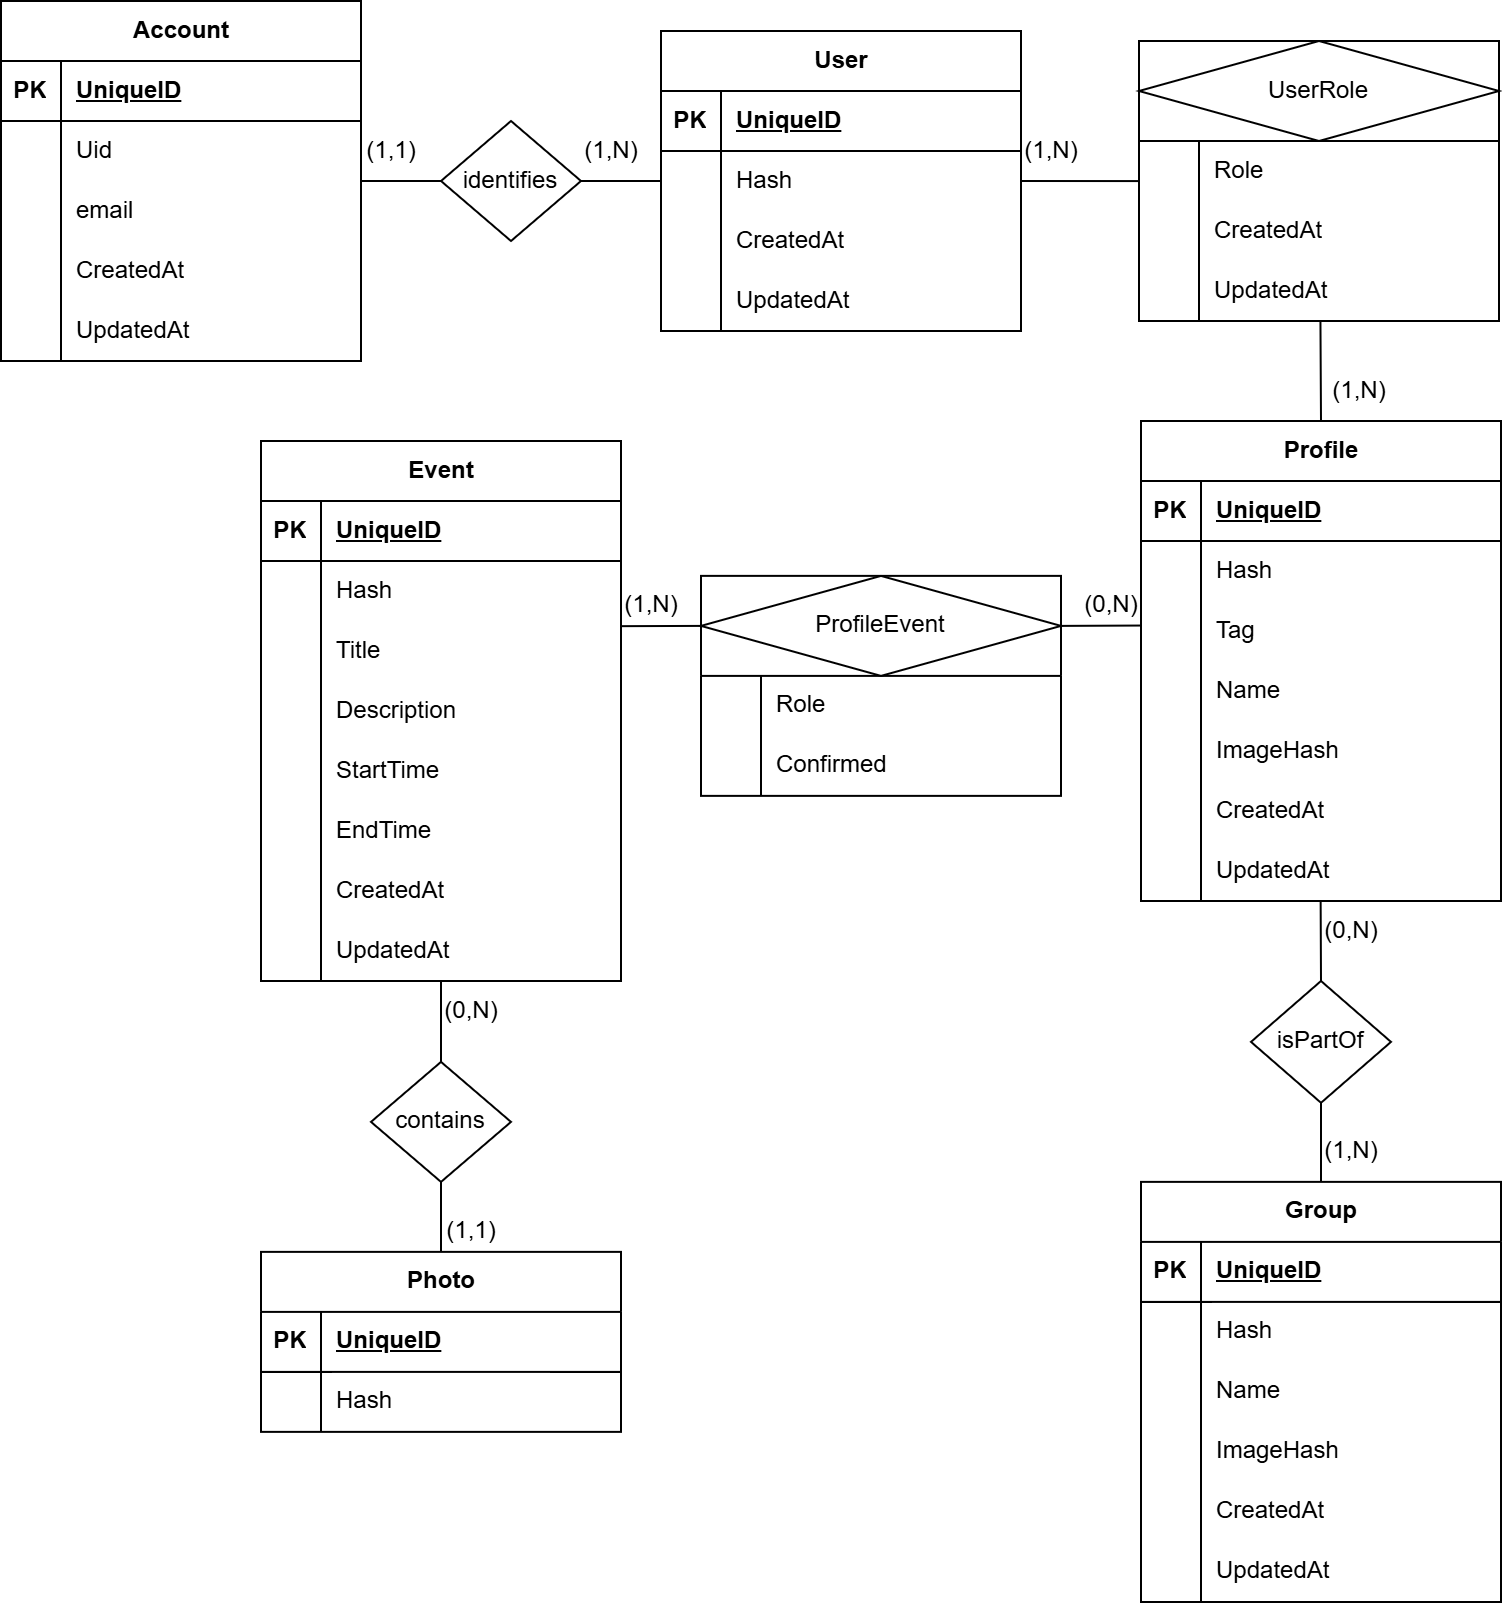
\includegraphics[width=\textwidth]{ProgettoDiagrammaER.png}
    \caption{Diagramma Entità - Relzione del dominio}
\end{figure}

Si creano quindi sul server le classi logiche del programma, a partire dal dominio.
Ogni classe corrisponde ad un oggetto del dominio, presentando i valori e le relazioni dei componenti come attributi dell’oggetto.\\
\\
Entity Framework Core di .Net(EFCore) è una libreria di C\# che permette di unire le classi logiche del programma alle tabelle del database.
Fornisce un’astrazione logica del collegamento con il database e le richieste relative, fornendo una rappresentazione di alto livello delle connessioni sottostanti. \\
\\
Una volta collegato il server con il database tramite le stringhe di connessione salvate sull’Azure Key Vault,
sono state definite le proprietà tra le varie entità, per poi inizializzare in automatico la struttura del database.
Le modifiche alla struttura del database vengono infatti generate automaticamente da EFCore in seguito alla creazione o alla modifica degli attributi degli oggetti.
Questo permette di star dietro agli aggiornamenti, generando e salvando le modifiche da applicare ad ogni modifica delle proprietà del dominio.\\
\\
\begin{figure}[h!]
    \begin{center}
        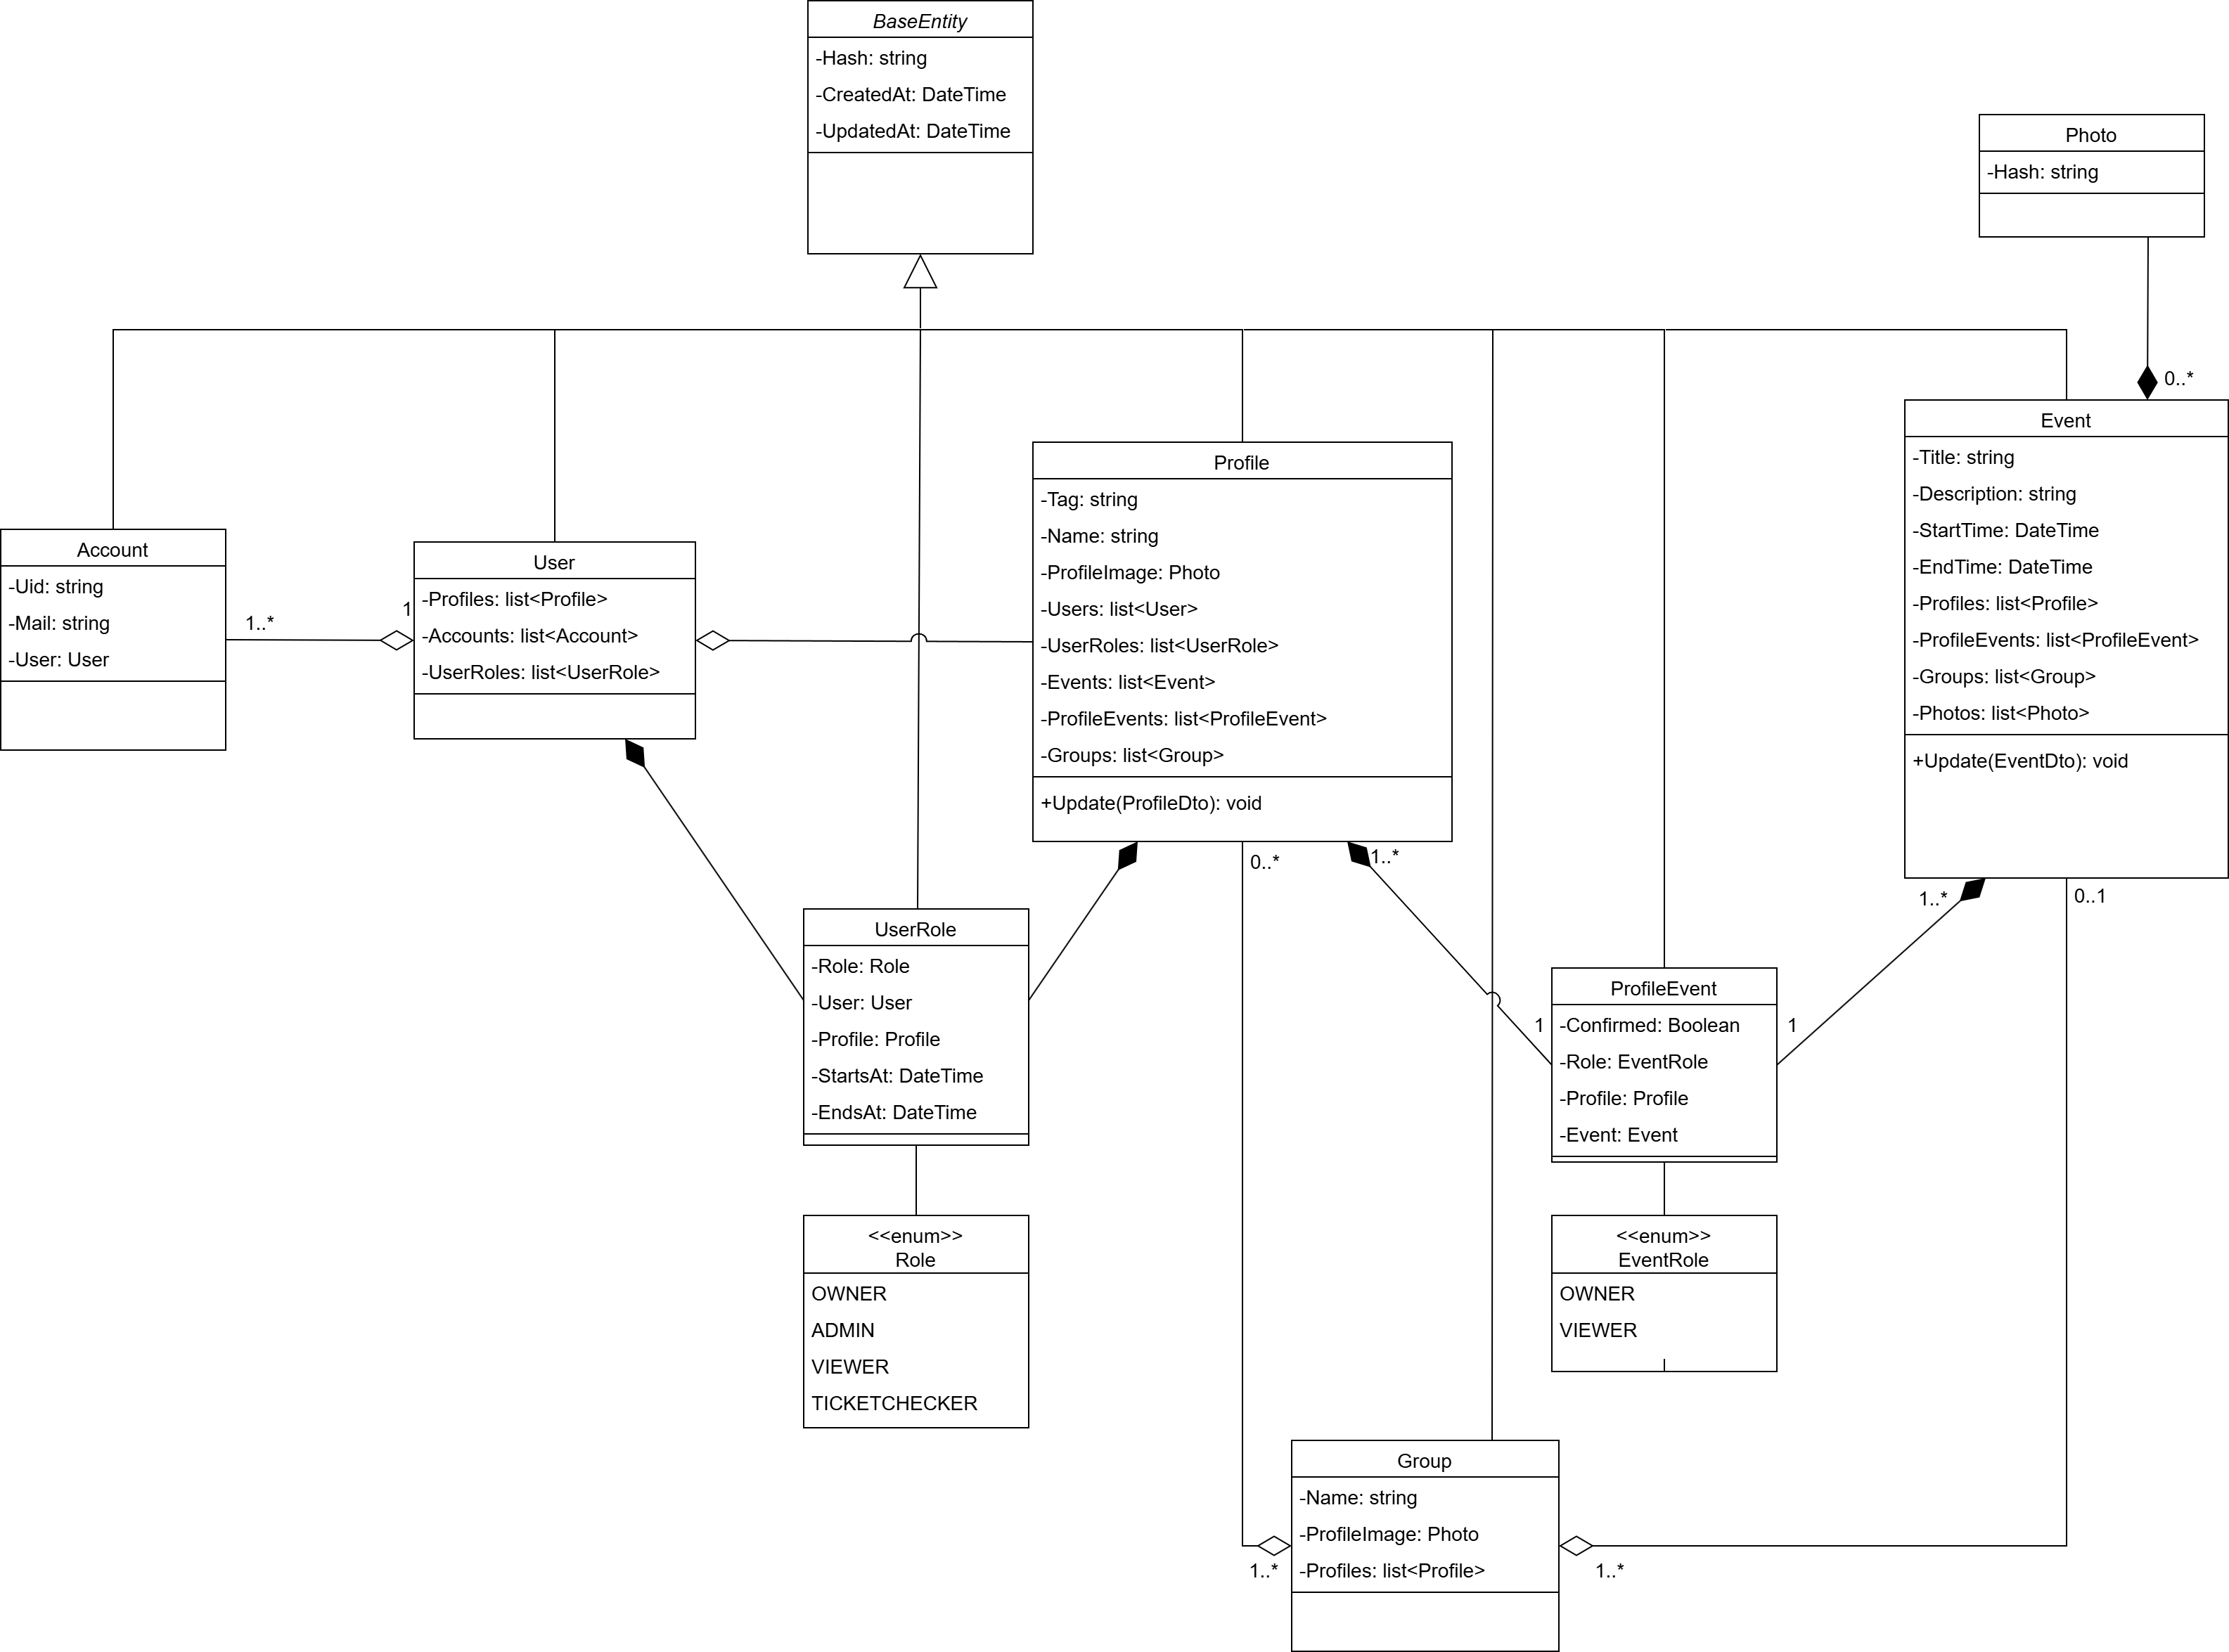
\includegraphics[width=\textwidth]{ModelClassDiagram.png}
        \caption{Modello delle classi del client}
    \end{center}
\end{figure}

Per la riduzione del carico computazionale richiesto da elementi con tante relazioni si utilizza la tecnica del lazy loading.
La tecnica del Lazy Loading consiste nel richiedere i dati delle relazioni di un elemento solo quando strettamente necessario.
La sua realizzazione tramite EFCore è attuata grazie alla proprietà virtual,
che permette di gestire un oggetto con un riferimento al database richiedendo i dati delle sue relazioni solo quando viene espressamente richiesto.
\clearpage